\documentclass[12pt]{article}

\usepackage{times}

% Packages I manually added
\usepackage{graphicx}
\usepackage{placeins}
\usepackage{float}
\usepackage{amsmath}
\usepackage{hyperref}
\usepackage{pdflscape}

%%% The "real" document content comes below...

\title{Behavioral changes in fleet dynamics due to MPAs}
\author{The Author}
%\date{} % Activate to display a given date or no date (if empty),
         % otherwise the current date is printed 

\begin{document}
\maketitle

\begin{abstract}
A
\end{abstract}

\section{Placeholder here}

ENSO events are known to drive the location of fish and the behavior of fishing vessels, especially in PNA waters \cite{lehodey_1997,kroodsma_2018,aqorau_2018}. We do our best to control for these environmental changes by incorporating the NINO4 anomaly index in our analyses, and by tracking the non-displaced vessels as a ``control'' group that is equally affected by the environmental variation. For example, we observe that both displaced and non-displaced vessels shifted their effort post-PIPA to the Western margin of the PNA region, namely Kiribati's Gilbert Islands and Tuvalu. However, displaced vessels redistribute a greater proportion of fishing effort to these areas, as well as the High Seas (Fig \ref{fig:fishing_raster_diff}). Our analysis shows that sea surface temperature variation does have an effect on our crowding and behavioral outcomes, but that by itself it does not explain the observed patterns. While environmental variation certainly influences fishing behavior, policy and management interventions such as moratoriums and spatial closures can have even larger effects \cite{kroodsma_2018}.  Our analyses incorporate the monthly NINO4 anomaly index (Fig. \ref{fig:nino_plot}) to control for the responses that fish and vessels might have to environmental variation \cite{lehodey_1997,kroodsma_2018,aqorau_2018}.

\begin{figure}
\centering
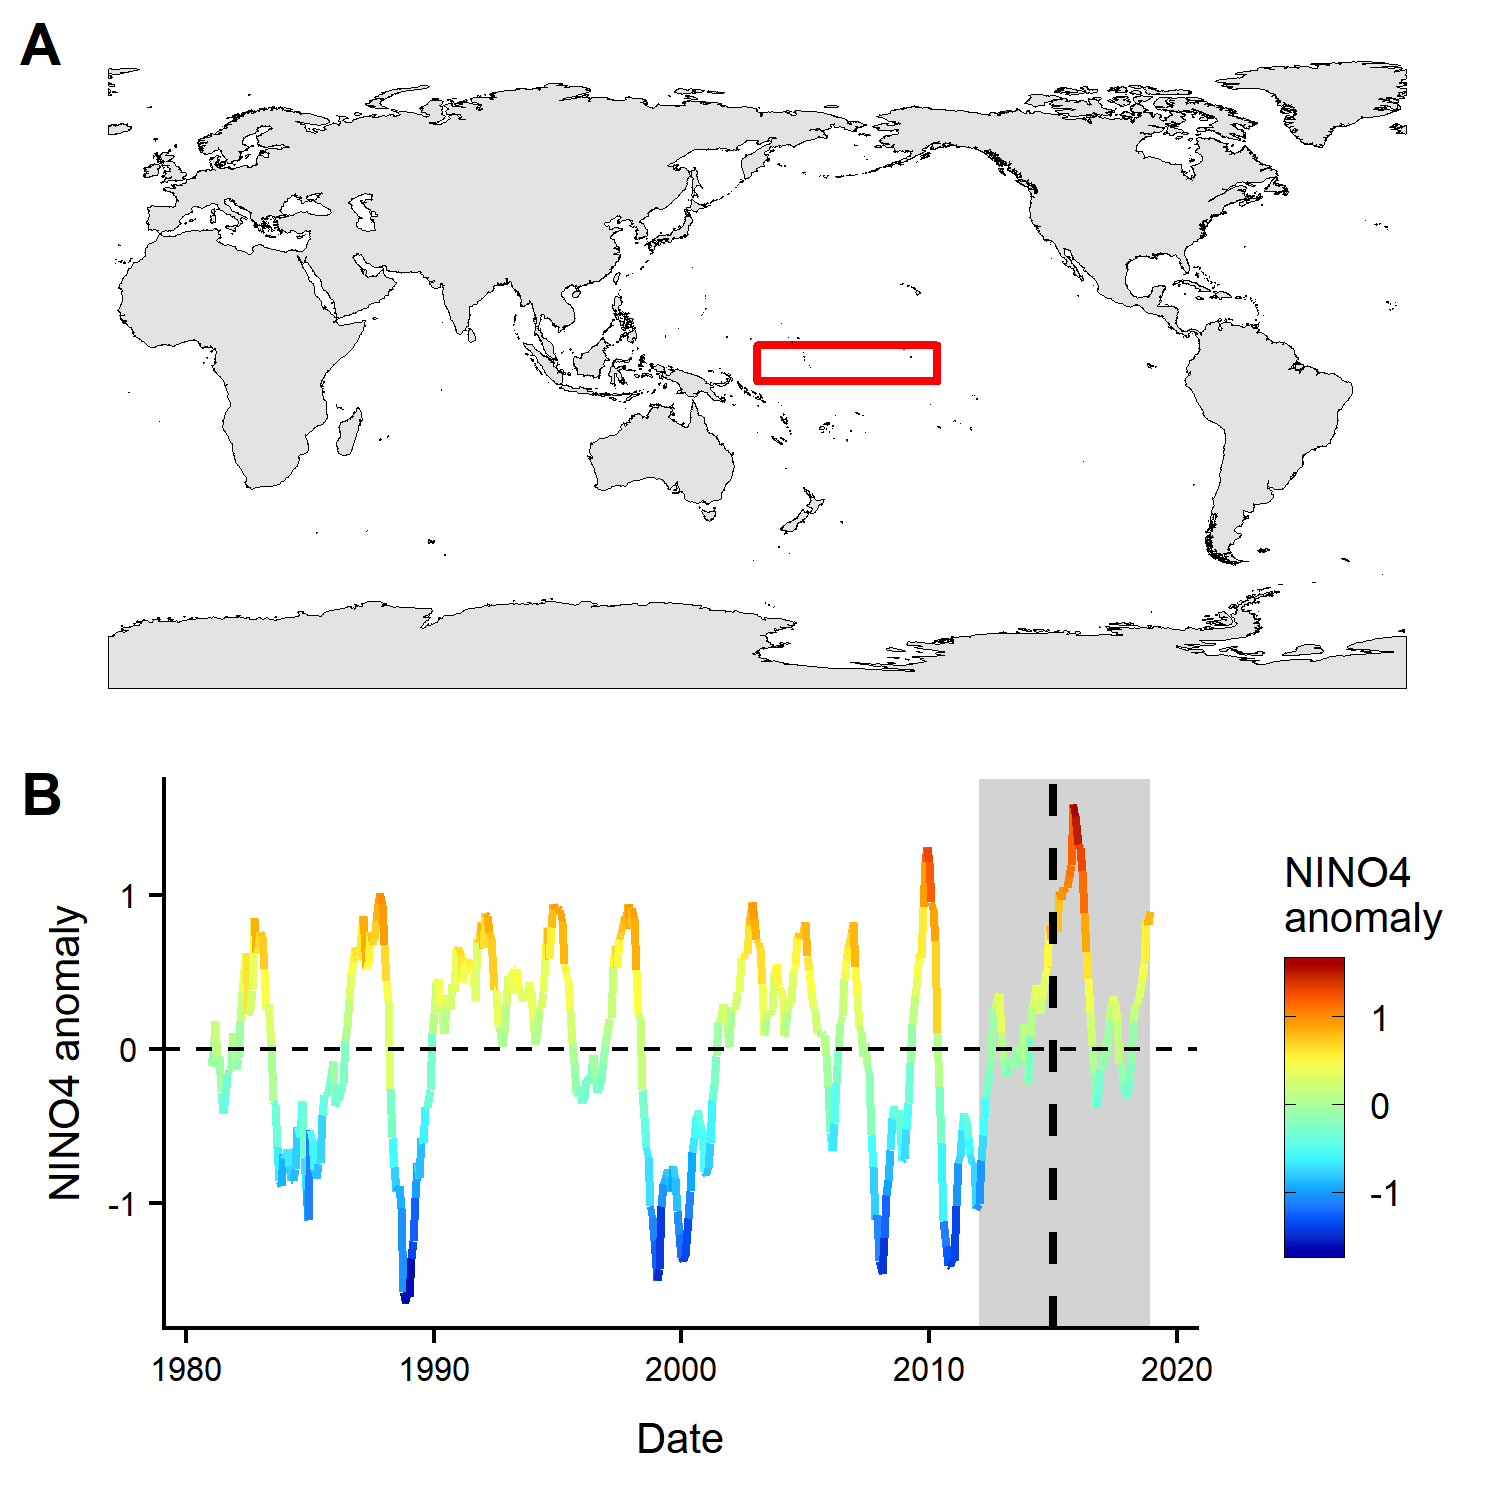
\includegraphics{img/nino_plot.png}
\caption{\label{fig:nino_plot}NINO4 anomaly index. A) Map of the NINO4 region (5S-5N and 160E-150W). B) Time series of NINO4 anomaly from January, 1980 to December, 2018.}
\end{figure}

\subsubsection{Behavioral changes}

We attempt to identify the response of vessels to the PIPA closure. We use daily fishing and non-fishing hours, daily proportion of fishing vs. non-fishing hours, daily distance traveled (km), distance from shore (km) and distance from home port (km) for fishing events, and proportion of total fishing hours allocated to Kiribati waters and PNA waters as our main outcomes of interest (Figure \ref{fig:all_panels}). We compare these outcomes before and after the implementation of PIPA using a Difference-in-Differences approach.

Our main specification is the following:

$$
log(y_{i,t}) = \alpha + \beta_1 P_t + \beta_2 D_i + \beta_3 P_t \times D_i + \phi_t + \gamma_i + \epsilon_{i,t}
\label{eqn:did}
$$

\noindent where $log(y_{i,t})$ is the hyperbolic-sine transformation\footnote{$ln\left(y + \sqrt{1 + y^2}\right)\rightarrow ln(2y)$. The transformation was not applied to the proportion of fishing to non-fishing hours.} of the outcome of interest for vessel $i$ in period $t$. A dummy variable $P_t$ takes the value of 0 for all dates prior to PIPA implementation and a value of 1 for all dates following PIPA implementation. $D_i$ is a dummy variable indicating whether a vessel belongs to the displaced ($D_i = 1$) or non-displaced ($D_i = 0$) group. $\alpha$ is the standard intercept term, $\beta_1$ captures the temporal trend, $\beta_2$ captures the initial difference between displaced and non-displaced groups, and $\beta_3$ is our parameter of interest: the difference-in-differences estimate capturing the treatment effect. Finally, $\phi_t$ and $\gamma_i$ represent month and flag dummies that account for seasonality or country-level management interventions. All regression coefficients were estimated via ordinary least squares, and heteroskedasticity-robust standard errors were calculated (Table \ref{tab:main_DID}).

We find no evidence of displaced vessels fishing more after the implementation and, in fact, observe a 27.5\% decrease relative to non-displaced vessels ($p < 0.01$; Fig. \ref{fig:all_panels}; Table \ref{tab:main_DID}). Likewise, we observe a 3.4\% decrease in fishing hours relative to total at-sea hours ($p < 0.01$). Displaced vessels traveled 23.3\% less distance, and fishing events occurred 32.9\% and 16.9\% closer to shore and to port, respectively. These changes in distance from shore and port are likely explained by redistribution, as we observe that displaced vessels fished less in Kiribati and PNA waters, compared to the trend observed for non-displaced vessels ($p < 0.01$). We do not observe changes in non-fishing at-sea hours (\emph{i.e.} a proxy for search time) and fishing hours on the High Seas. We repeat this analysis for sample restrictions where we exclude all Chinese vessels (Table \ref{tab:DID_without_CHN}), all PNA-owned vessels (Table \ref{tab:DID_without_PNA}) and all Taiwanese and USA vessels (Table \ref{tab:DID_without_USA_TWN}) and find qualitatively the same responses.

\begin{landscape}
\begin{table}[H] \centering 
  \caption{\label{tab:main_DID}Difference-in-differences estimates for our 9 variables of interest: 1) Daily fishing hours, 2) Daily non-fishing at-sea hours, 3) Daily proportion of fishing hours to total at-sea hours, 4) Daily distance traveled, 5) Daily mean distance from port for fishing events, 6) Daily mean distance from shore for fishing events, 7) Monthly fishing hours spent in Kiribati waters, 8) Monthly fishing hours spent in PNA waters, and 9) Monthly fishing hours in the high seas. Numbers in parentheses are heteroskedastic-robust standard errors.} 
  \label{} 
\footnotesize 
\begin{tabular}{@{\extracolsep{1pt}}lccccccccc} 
\\[-1.8ex]\hline 
\hline \\[-1.8ex] 
\\[-1.8ex] & (1) & (2) & (3) & (4) & (5) & (6) & (7) & (8) & (9)\\ 
\hline \\[-1.8ex] 
 Constant & 0.495$^{***}$ & 3.607$^{***}$ & 0.075$^{***}$ & 4.440$^{***}$ & 12.998$^{***}$ & 12.462$^{***}$ & 3.709$^{***}$ & 4.456$^{***}$ & 2.429$^{***}$ \\ 
  & (0.022) & (0.012) & (0.004) & (0.042) & (0.021) & (0.019) & (0.195) & (0.151) & (0.415) \\ 
  & & & & & & & & & \\ 
 Post & 0.846$^{***}$ & $-$0.227$^{***}$ & 0.138$^{***}$ & 0.112$^{***}$ & 0.271$^{***}$ & 0.275$^{***}$ & 0.943$^{***}$ & 1.129$^{***}$ & 0.709$^{**}$ \\ 
  & (0.018) & (0.009) & (0.003) & (0.031) & (0.014) & (0.014) & (0.141) & (0.110) & (0.284) \\ 
  & & & & & & & & & \\ 
 Displaced & 0.136$^{***}$ & 0.014$^{**}$ & 0.015$^{***}$ & 0.255$^{***}$ & 0.225$^{***}$ & 0.117$^{***}$ & 0.549$^{***}$ & 0.153 & $-$0.280 \\ 
  & (0.013) & (0.007) & (0.002) & (0.029) & (0.016) & (0.016) & (0.148) & (0.118) & (0.236) \\ 
  & & & & & & & & & \\ 
 NINO4 & $-$0.014 & $-$0.001 & $-$0.001 & $-$0.411$^{***}$ & 0.167$^{***}$ & 0.064$^{***}$ & 0.357$^{***}$ & 0.137$^{**}$ & 0.484$^{***}$ \\ 
  & (0.011) & (0.005) & (0.002) & (0.017) & (0.008) & (0.007) & (0.068) & (0.056) & (0.122) \\ 
  & & & & & & & & & \\ 
 Post $\times$ Displaced & $-$0.243$^{***}$ & 0.013 & $-$0.034$^{***}$ & $-$0.210$^{***}$ & $-$0.285$^{***}$ & $-$0.157$^{***}$ & $-$0.586$^{***}$ & $-$0.403$^{***}$ & 0.338 \\ 
  & (0.019) & (0.009) & (0.003) & (0.036) & (0.017) & (0.017) & (0.161) & (0.127) & (0.285) \\ 
  & & & & & & & & & \\ 
\hline \\[-1.8ex] 
Month FE & Yes & Yes & Yes & Yes & Yes & Yes & Yes & Yes & Yes \\ 
Flag FE & Yes & Yes & Yes & Yes & Yes & Yes & Yes & Yes & Yes \\ 
Observations & 83,052 & 83,052 & 83,051 & 79,669 & 32,055 & 32,055 & 1,814 & 2,588 & 684 \\ 
R$^{2}$ & 0.102 & 0.072 & 0.107 & 0.017 & 0.075 & 0.082 & 0.126 & 0.200 & 0.252 \\ 
\hline 
\hline \\[-1.8ex] 
\textit{Note:}  & \multicolumn{9}{r}{$^{*}$p$<$0.1; $^{**}$p$<$0.05; $^{***}$p$<$0.01} \\ 
\end{tabular} 
\end{table} 
\end{landscape}

\begin{figure}
	\centering
	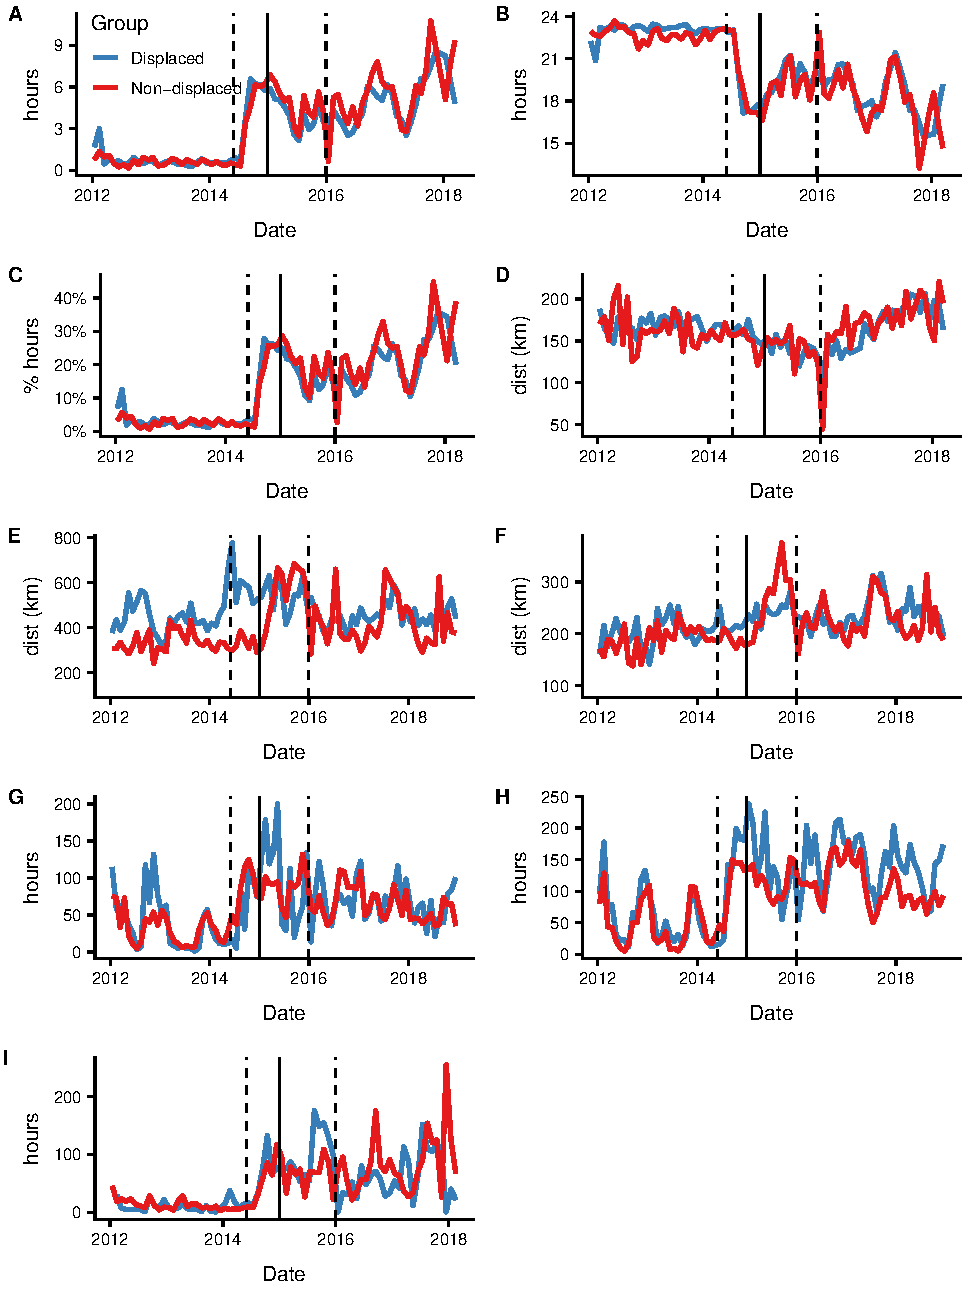
\includegraphics{img/all_panels.pdf}
	\caption{\label{fig:all_panels}Time series showing monthly averages for our nine variables of interest: A) Fishing hours, B) Non-fishing hours at-sea, C) Proportion of fishing hours to total hours at-sea, D) Distance traveled, E) Mean distance from port for fishing events, F) Mean distance from shore for fishing events, G) Monthly hours spent in Kiribati waters, H) Monthly hours spent in PNA waters, I) Monthly hours spent on the high seas. Dashed vertical lines indicate the addition of new AIS satellites. Solid vertical line indicates the closure of PIPA.}
\end{figure}

\begin{figure}
	\centering
	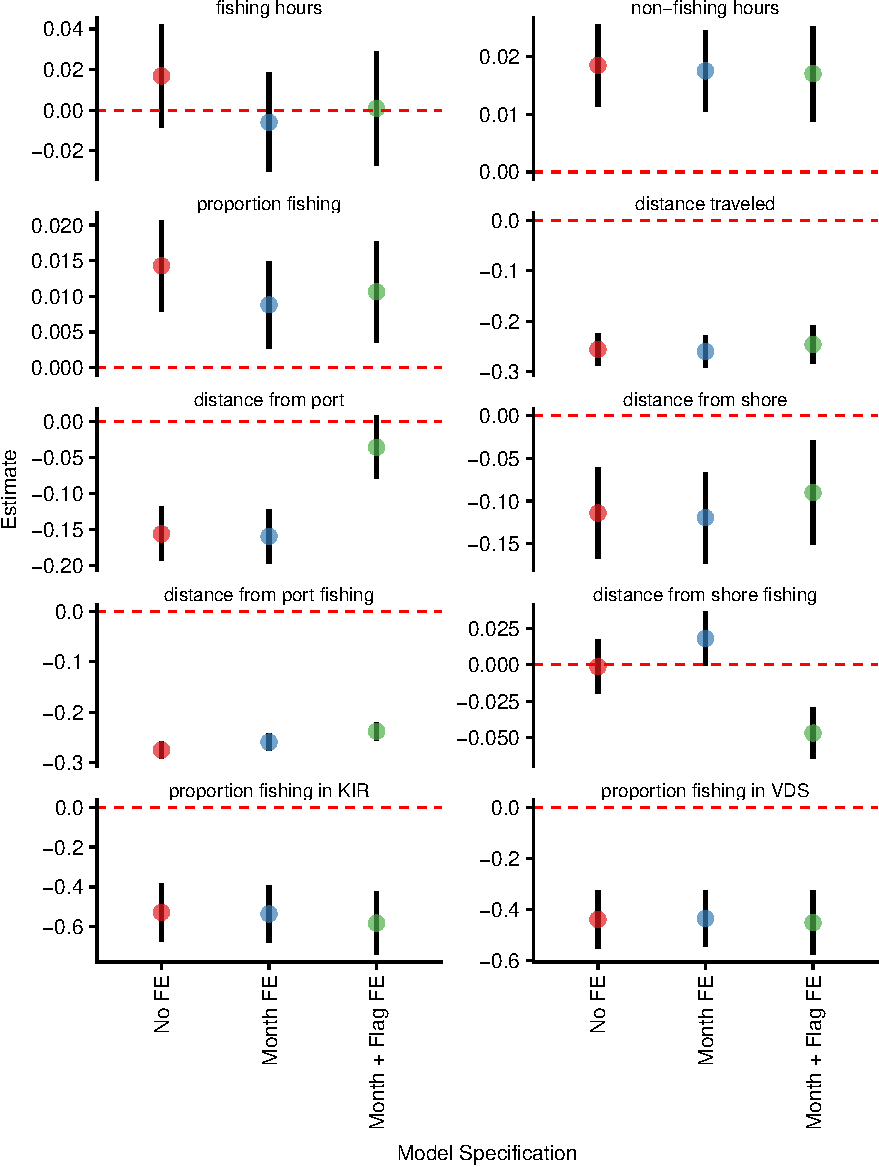
\includegraphics{img/other_specifications.pdf}
	\caption{\label{fig:other_specifications}Alternative difference-in-differences estimates for our variables of interest using different model specifications. Table \ref{tab:main_DID} reports estimates for models with month and flag fixed effects, and NINO4 index (\emph{i.e.} green dots).}
\end{figure}

\begin{landscape}
\begin{table}[H] \centering 
  \caption{\label{tab:DID_without_CHN}Difference-in-differences estimates for our 9 variables of interest after removing Chinese vessels. 1) Daily fishing hours, 2) Daily non-fishing at-sea hours, 3) Daily proportion of fishing hours to total at-sea hours, 4) Daily distance traveled, 5) Daily mean distance from port for fishing events, 6) Daily mean distance from shore for fishing events, 7) Monthly fishing hours spent in Kiribati waters, 8) Monthly fishing hours spent in PNA waters, and 9) Monthly fishing hours in the high seas. Numbers in parentheses are heteroskedastic-robust standard errors.} 
  \label{} 
\footnotesize 
\begin{tabular}{@{\extracolsep{1pt}}lccccccccc} 
\\[-1.8ex]\hline 
\hline \\[-1.8ex] 
\\[-1.8ex] & (1) & (2) & (3) & (4) & (5) & (6) & (7) & (8) & (9)\\ 
\hline \\[-1.8ex] 
 Constant & 0.058$^{***}$ & 3.863$^{***}$ & $-$0.003 & 4.829$^{***}$ & 13.817$^{***}$ & 13.161$^{***}$ & 4.007$^{***}$ & 4.515$^{***}$ & 2.909$^{***}$ \\ 
  & (0.019) & (0.008) & (0.003) & (0.044) & (0.044) & (0.058) & (0.347) & (0.304) & (0.274) \\ 
  & & & & & & & & & \\ 
 Post & 0.824$^{***}$ & $-$0.254$^{***}$ & 0.136$^{***}$ & 0.145$^{***}$ & 0.306$^{***}$ & 0.322$^{***}$ & 0.920$^{***}$ & 1.157$^{***}$ & 0.691$^{**}$ \\ 
  & (0.019) & (0.010) & (0.003) & (0.034) & (0.016) & (0.016) & (0.156) & (0.121) & (0.291) \\ 
  & & & & & & & & & \\ 
 Displaced & 0.108$^{***}$ & 0.009 & 0.012$^{***}$ & 0.270$^{***}$ & 0.271$^{***}$ & 0.158$^{***}$ & 0.491$^{***}$ & 0.150 & $-$0.274 \\ 
  & (0.013) & (0.007) & (0.002) & (0.031) & (0.017) & (0.017) & (0.162) & (0.131) & (0.235) \\ 
  & & & & & & & & & \\ 
 NINO4 & $-$0.012 & $-$0.007 & $-$0.001 & $-$0.380$^{***}$ & 0.164$^{***}$ & 0.061$^{***}$ & 0.365$^{***}$ & 0.122$^{**}$ & 0.464$^{***}$ \\ 
  & (0.011) & (0.005) & (0.002) & (0.018) & (0.009) & (0.008) & (0.074) & (0.060) & (0.126) \\ 
  & & & & & & & & & \\ 
 Post $\times$ Displaced & $-$0.212$^{***}$ & 0.040$^{***}$ & $-$0.031$^{***}$ & $-$0.282$^{***}$ & $-$0.338$^{***}$ & $-$0.205$^{***}$ & $-$0.558$^{***}$ & $-$0.412$^{***}$ & 0.374 \\ 
  & (0.021) & (0.010) & (0.004) & (0.038) & (0.019) & (0.018) & (0.174) & (0.137) & (0.289) \\ 
  & & & & & & & & & \\ 
\hline \\[-1.8ex] 
Month FE & Yes & Yes & Yes & Yes & Yes & Yes & Yes & Yes & Yes \\ 
Flag FE & Yes & Yes & Yes & Yes & Yes & Yes & Yes & Yes & Yes \\ 
Observations & 75,327 & 75,327 & 75,326 & 75,390 & 28,449 & 28,449 & 1,570 & 2,279 & 633 \\ 
R$^{2}$ & 0.102 & 0.073 & 0.108 & 0.017 & 0.075 & 0.091 & 0.128 & 0.209 & 0.266 \\ 
\hline 
\hline \\[-1.8ex] 
\textit{Note:}  & \multicolumn{9}{r}{$^{*}$p$<$0.1; $^{**}$p$<$0.05; $^{***}$p$<$0.01} \\ 
\end{tabular} 
\end{table} 
\end{landscape}

\begin{landscape}
\begin{table}[H] \centering 
  \caption{\label{tab:DID_without_PNA}Difference-in-differences estimates for our 9 variables of interest after removing PNA vessels: 1) Daily fishing hours, 2) Daily non-fishing at-sea hours, 3) Daily proportion of fishing hours to total at-sea hours, 4) Daily distance traveled, 5) Daily mean distance from port for fishing events, 6) Daily mean distance from shore for fishing events, 7) Monthly fishing hours spent in Kiribati waters, 8) Monthly fishing hours spent in PNA waters, and 9) Monthly fishing hours in the high seas. Numbers in parentheses are heteroskedastic-robust standard errors.} 
  \label{} 
\footnotesize 
\begin{tabular}{@{\extracolsep{1pt}}lccccccccc} 
\\[-1.8ex]\hline 
\hline \\[-1.8ex] 
\\[-1.8ex] & (1) & (2) & (3) & (4) & (5) & (6) & (7) & (8) & (9)\\ 
\hline \\[-1.8ex] 
 Constant & 0.512$^{***}$ & 3.559$^{***}$ & 0.083$^{***}$ & 4.499$^{***}$ & 13.165$^{***}$ & 12.667$^{***}$ & 3.271$^{***}$ & 4.066$^{***}$ & 2.876$^{***}$ \\ 
  & (0.024) & (0.013) & (0.004) & (0.047) & (0.028) & (0.025) & (0.263) & (0.201) & (0.434) \\ 
  & & & & & & & & & \\ 
 Post & 0.781$^{***}$ & $-$0.159$^{***}$ & 0.122$^{***}$ & 0.047 & 0.114$^{***}$ & 0.070$^{***}$ & 1.168$^{***}$ & 1.481$^{***}$ & 0.295 \\ 
  & (0.022) & (0.012) & (0.004) & (0.043) & (0.023) & (0.022) & (0.226) & (0.180) & (0.333) \\ 
  & & & & & & & & & \\ 
 Displaced & 0.202$^{***}$ & 0.040$^{***}$ & 0.019$^{***}$ & 0.437$^{***}$ & 0.165$^{***}$ & $-$0.015 & 0.817$^{***}$ & 0.533$^{***}$ & $-$0.408$^{*}$ \\ 
  & (0.015) & (0.009) & (0.003) & (0.037) & (0.024) & (0.022) & (0.229) & (0.182) & (0.235) \\ 
  & & & & & & & & & \\ 
 NINO4 & $-$0.019 & $-$0.0003 & $-$0.002 & $-$0.387$^{***}$ & 0.138$^{***}$ & 0.025$^{***}$ & 0.413$^{***}$ & 0.232$^{***}$ & 0.482$^{***}$ \\ 
  & (0.012) & (0.006) & (0.002) & (0.020) & (0.010) & (0.009) & (0.080) & (0.066) & (0.156) \\ 
  & & & & & & & & & \\ 
 Post $\times$ Displaced & $-$0.219$^{***}$ & $-$0.055$^{***}$ & $-$0.023$^{***}$ & $-$0.246$^{***}$ & $-$0.175$^{***}$ & 0.010 & $-$0.843$^{***}$ & $-$0.821$^{***}$ & 0.729$^{**}$ \\ 
  & (0.024) & (0.012) & (0.004) & (0.046) & (0.026) & (0.024) & (0.243) & (0.195) & (0.341) \\ 
  & & & & & & & & & \\ 
\hline \\[-1.8ex] 
Month FE & Yes & Yes & Yes & Yes & Yes & Yes & Yes & Yes & Yes \\ 
Flag FE & Yes & Yes & Yes & Yes & Yes & Yes & Yes & Yes & Yes \\ 
Observations & 64,560 & 64,560 & 64,559 & 64,625 & 22,654 & 22,654 & 1,366 & 1,928 & 511 \\ 
R$^{2}$ & 0.093 & 0.069 & 0.099 & 0.022 & 0.063 & 0.066 & 0.127 & 0.203 & 0.214 \\ 
\hline 
\hline \\[-1.8ex] 
\textit{Note:}  & \multicolumn{9}{r}{$^{*}$p$<$0.1; $^{**}$p$<$0.05; $^{***}$p$<$0.01} \\ 
\end{tabular} 
\end{table} 
\end{landscape}

\begin{landscape}
\begin{table}[H] \centering 
  \caption{\label{tab:DID_without_USA_TWN}Difference-in-differences estimates for our 9 variables of interest after removing US and Tawianese vessels. 1) Daily fishing hours, 2) Daily non-fishing at-sea hours, 3) Daily proportion of fishing hours to total at-sea hours, 4) Daily distance traveled, 5) Daily mean distance from port for fishing events, 6) Daily mean distance from shore for fishing events, 7) Monthly fishing hours spent in Kiribati waters, 8) Monthly fishing hours spent in PNA waters, and 9) Monthly fishing hours in the high seas. Numbers in parentheses are heteroskedastic-robust standard errors.} 
  \label{} 
\footnotesize 
\begin{tabular}{@{\extracolsep{1pt}}lccccccccc} 
\\[-1.8ex]\hline 
\hline \\[-1.8ex] 
\\[-1.8ex] & (1) & (2) & (3) & (4) & (5) & (6) & (7) & (8) & (9)\\ 
\hline \\[-1.8ex] 
 Constant & 0.536$^{***}$ & 3.600$^{***}$ & 0.082$^{***}$ & 4.506$^{***}$ & 13.002$^{***}$ & 12.438$^{***}$ & 3.850$^{***}$ & 4.719$^{***}$ & 2.420$^{***}$ \\ 
  & (0.023) & (0.012) & (0.004) & (0.043) & (0.022) & (0.020) & (0.209) & (0.158) & (0.419) \\ 
  & & & & & & & & & \\ 
 Post & 0.796$^{***}$ & $-$0.217$^{***}$ & 0.130$^{***}$ & 0.021 & 0.290$^{***}$ & 0.291$^{***}$ & 0.870$^{***}$ & 0.894$^{***}$ & 0.732$^{**}$ \\ 
  & (0.019) & (0.010) & (0.003) & (0.035) & (0.016) & (0.016) & (0.156) & (0.121) & (0.291) \\ 
  & & & & & & & & & \\ 
 Displaced & 0.142$^{***}$ & 0.016$^{**}$ & 0.015$^{***}$ & 0.341$^{***}$ & 0.227$^{***}$ & 0.127$^{***}$ & 0.490$^{***}$ & $-$0.017 & $-$0.296 \\ 
  & (0.013) & (0.007) & (0.002) & (0.031) & (0.018) & (0.017) & (0.163) & (0.126) & (0.239) \\ 
  & & & & & & & & & \\ 
 NINO4 & $-$0.001 & $-$0.001 & 0.001 & $-$0.383$^{***}$ & 0.189$^{***}$ & 0.082$^{***}$ & 0.325$^{***}$ & 0.171$^{***}$ & 0.441$^{***}$ \\ 
  & (0.011) & (0.006) & (0.002) & (0.019) & (0.009) & (0.008) & (0.075) & (0.063) & (0.122) \\ 
  & & & & & & & & & \\ 
 Post $\times$ Displaced & $-$0.212$^{***}$ & $-$0.002 & $-$0.029$^{***}$ & $-$0.158$^{***}$ & $-$0.328$^{***}$ & $-$0.184$^{***}$ & $-$0.533$^{***}$ & $-$0.225 & 0.339 \\ 
  & (0.021) & (0.010) & (0.004) & (0.039) & (0.019) & (0.018) & (0.175) & (0.138) & (0.291) \\ 
  & & & & & & & & & \\ 
\hline \\[-1.8ex] 
Month FE & Yes & Yes & Yes & Yes & Yes & Yes & Yes & Yes & Yes \\ 
Flag FE & Yes & Yes & Yes & Yes & Yes & Yes & Yes & Yes & Yes \\ 
Observations & 73,717 & 73,717 & 73,716 & 73,778 & 26,920 & 26,920 & 1,546 & 2,236 & 660 \\ 
R$^{2}$ & 0.095 & 0.072 & 0.102 & 0.021 & 0.077 & 0.094 & 0.111 & 0.169 & 0.256 \\ 
\hline 
\hline \\[-1.8ex] 
\textit{Note:}  & \multicolumn{9}{r}{$^{*}$p$<$0.1; $^{**}$p$<$0.05; $^{***}$p$<$0.01} \\ 
\end{tabular} 
\end{table} 
\end{landscape}

\subsubsection{Crowding effect}

\begin{equation}
y_t = \alpha + \beta_1 M_t + \beta_2 M_t^2 + \beta_3 M_t^3 + \beta_4 M_t ^4 + \sigma_s + \mu N_t + \epsilon_t
\label{eqn:sp_corr}
\end{equation}

We test for a crowding effect using the specification in Equation \ref{eqn:sp_corr}. We have two different outcome variables:
1) the number of cells that had fishing activity from displaced and non-displaced vessels per month and 2) the correlation of presence/absence of fishing events between both groups over one month.We allow for the possibility of three inflection points: 1) initial crowding due to MPA implementation, 2) When the crowding has reached its peak and starts to decrease, and 3) when this decrease potentially levels off. For this reason, we fit a 4th degree polynomial to our monthly indices. We do so by centering our time series of crowding indices on the day of implementation. Our explanatory variable is therefore the number of months ($M$) before or after the implementation. For example, since PIPA was implemented on January 1\textsuperscript{st} of 2015, December of 2014 has a value of -1 and Feb of 2015 would receive a value of 1. Note that we restrict the sample to our displaced and non-displaced vessels (vessels that show up in the dataset before PIPA implementation) to try to minimize bias from more and more vessels using AIS over time. We also include controls ($\sigma_s$) that captures the effect of additional satellites receiving AIS signals, which occurred on April 1st, 2014 and December 31st, 2015. The $\mu$ coefficient captures the effect of the NINO4 anomaly.

We inspect the crowding effects that may arise by applying more (or the same) fishing effort over less fishing area by inspecting the spatial overlap between displaced and non-displaced vessels over a gridded surface (Fig \ref{fig:fishing_raster_diff}). These groups interacted more with each other after the implementation of PIPA (Table \ref{tab:sp_corr}, Fig. \ref{fig:sp_corr}). The number of cells with presence from both fleets and the spatial correlation between groups increases by a factor of four and three, respectively. Environmental variation may certainly drive this, but the NINO4 anomaly alone explained just 3\% and 7\% of the variation in our crowding measures, compared to the 70\% variation explained when accounting for PIPA implementation (Table \ref{tab:sp_corr}). We observe similar patterns when replicating the crowding exercise for Kiribati's EEZ only (Table \ref{tab:KIR_sp_corr}, Fig \ref{fig:KIR_sp_corr}).

\begin{landscape}
\begin{table}[H] \centering 
  \caption{\label{tab:sp_corr}Coefficient estimates for a fourth-degree polynomial fit to the measures of crowding for all PNA waters. The first five columns represent different specifications for number of cells with presence of both fleets. Columns 6 - 10 show coefficients for the spatial correlation for presence / absence of displaced and non-displaced vessels. The explanatory variable is the number of months before or after implementation of PIPA. Numbers in parentheses are heteroskedastic-robust standard errors. The last column of each group presents fits with only NINO4 anomaly index as an explanatory variable.} 
  \label{} 
\footnotesize 
\begin{tabular}{@{\extracolsep{0.1pt}}lcccccccccc} 
\\[-1.8ex]\hline 
\hline \\[-1.8ex] 
\\[-1.8ex] & \multicolumn{5}{c}{Number of cells} & \multicolumn{5}{c}{Pearson's correlation coefficient} \\ 
\\[-1.8ex] & (1) & (2) & (3) & (4) & (5) & (6) & (7) & (8) & (9) & (10)\\ 
\hline \\[-1.8ex] 
 Constant & 78.04$^{***}$ & 84.64$^{***}$ & 60.96$^{***}$ & 66.73$^{***}$ & 80.62$^{***}$ & 0.41$^{***}$ & 0.42$^{***}$ & 0.37$^{***}$ & 0.38$^{***}$ & 0.38$^{***}$ \\ 
  & (5.44) & (8.99) & (15.60) & (15.99) & (7.96) & (0.01) & (0.03) & (0.06) & (0.07) & (0.02) \\ 
  & & & & & & & & & & \\ 
 M & 3.94$^{***}$ & 4.07$^{***}$ & 3.07$^{***}$ & 3.14$^{***}$ &  & 0.01$^{***}$ & 0.01$^{***}$ & 0.01$^{**}$ & 0.01$^{**}$ &  \\ 
  & (0.30) & (0.35) & (0.97) & (1.04) &  & (0.001) & (0.001) & (0.003) & (0.004) &  \\ 
  & & & & & & & & & & \\ 
 M $^2$ & $-$0.005 & $-$0.02 & 0.01 & $-$0.01 &  & $-$0.0001$^{***}$ & $-$0.0001 & $-$0.0001 & $-$0.0001 &  \\ 
  & (0.02) & (0.03) & (0.03) & (0.03) &  & (0.0000) & (0.0001) & (0.0001) & (0.0001) &  \\ 
  & & & & & & & & & & \\ 
 M $^3$ & $-$0.002$^{***}$ & $-$0.002$^{***}$ & $-$0.002$^{***}$ & $-$0.002$^{***}$ &  & $-$0.0000$^{***}$ & $-$0.0000$^{***}$ & $-$0.0000$^{***}$ & $-$0.0000$^{***}$ &  \\ 
  & (0.0003) & (0.0003) & (0.001) & (0.001) &  & (0.0000) & (0.0000) & (0.0000) & (0.0000) &  \\ 
  & & & & & & & & & & \\ 
 M $^4$ & 0.0000 & 0.0000 & 0.0000 & 0.0000 &  & 0.0000$^{***}$ & 0.0000$^{**}$ & 0.0000 & 0.0000 &  \\ 
  & (0.0000) & (0.0000) & (0.0000) & (0.0000) &  & (0.0000) & (0.0000) & (0.0000) & (0.0000) &  \\ 
  & & & & & & & & & & \\ 
 NINO4 &  & $-$8.09 &  & $-$10.39 & 19.76$^{**}$ &  & $-$0.01 &  & $-$0.01 & 0.07$^{***}$ \\ 
  &  & (8.29) &  & (9.48) & (9.41) &  & (0.03) &  & (0.03) & (0.02) \\ 
  & & & & & & & & & & \\ 
 $\sigma_1$ &  &  & 21.32 & 25.10 &  &  &  & 0.06 & 0.06 &  \\ 
  &  &  & (19.49) & (22.49) &  &  &  & (0.08) & (0.08) &  \\ 
  & & & & & & & & & & \\ 
 $\sigma_2$ &  &  & 5.30 & 3.19 &  &  &  & $-$0.01 & $-$0.02 &  \\ 
  &  &  & (18.87) & (18.67) &  &  &  & (0.04) & (0.03) &  \\ 
  & & & & & & & & & & \\ 
\hline \\[-1.8ex] 
NINO4 & No & Yes & No & Yes & Yes & No & Yes & No & Yes & Yes \\ 
Satellites & No & No & Yes & Yes & No &  &  &  &  &  \\ 
AIC & 796.937 & 797.991 & 799.477 & 799.97 & 919.583 & -187.208 & -185.269 & -184.916 & -183.233 & -97.386 \\ 
Observations & 84 & 84 & 84 & 84 & 84 & 84 & 84 & 84 & 84 & 84 \\ 
R$^{2}$ & 0.79 & 0.79 & 0.79 & 0.80 & 0.03 & 0.70 & 0.70 & 0.71 & 0.71 & 0.07 \\ 
\hline 
\hline \\[-1.8ex] 
\textit{Note:}  & \multicolumn{10}{r}{$^{*}$p$<$0.1; $^{**}$p$<$0.05; $^{***}$p$<$0.01} \\ 
\end{tabular} 
\end{table} 
\end{landscape}

\begin{figure}[htbp]
\centering
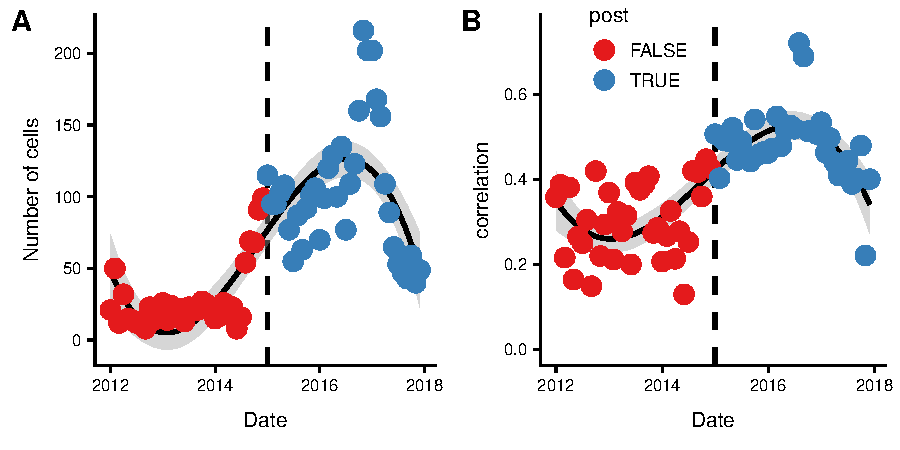
\includegraphics{img/sp_corr.pdf}
\caption{\label{fig:sp_corr}Number of cells that had displaced and non-displaced vessels (A) and spatial correlation in the presence-absence of each group per cell (B). The solid lines represent the 4\textsuperscript{th} degree polynomial fit reported in \ref{tab:sp_corr}. Note that the late 2016 and early 2017 showed negative or neutral NINO4 anomalies similar to those in the pre-PIPA period, but crowding effect does not decline to pre-implementation level and seems to stabilize.}
\end{figure}

\begin{landscape}
\begin{table}[H] \centering 
  \caption{\label{tab:KIR_sp_corr}Coefficient estimates for a fourth-degree polynomial fit to the measures of crowding for Kiribati EEZ only. The first five columns represent different specifications for number of cells with presence of both fleets. Columns 6 - 10 show coefficients for the spatial correlation for presence / absence of displaced and non-displaced vessels. The explanatory variable is the number of months before or after implementation of PIPA. Numbers in parentheses are heteroskedastic-robust standard errors. The last column of each group presents fits with only NINO4 anomaly index as an explanatory variable.} 
  \label{} 
\footnotesize 
\begin{tabular}{@{\extracolsep{0.1pt}}lcccccccccc} 
\\[-1.8ex]\hline 
\hline \\[-1.8ex] 
\\[-1.8ex] & \multicolumn{5}{c}{Number of cells} & \multicolumn{5}{c}{Pearson's correlation coefficient} \\ 
\\[-1.8ex] & (1) & (2) & (3) & (4) & (5) & (6) & (7) & (8) & (9) & (10)\\ 
\hline \\[-1.8ex] 
 Constant & 30.24$^{***}$ & 32.77$^{***}$ & 23.30$^{***}$ & 26.14$^{***}$ & 16.23$^{***}$ & 0.43$^{***}$ & 0.43$^{***}$ & 0.33$^{***}$ & 0.34$^{***}$ & 0.38$^{***}$ \\ 
  & (2.43) & (4.16) & (4.59) & (5.49) & (2.37) & (0.03) & (0.05) & (0.07) & (0.08) & (0.03) \\ 
  & & & & & & & & & & \\ 
 M & 1.29$^{***}$ & 1.34$^{***}$ & 1.00$^{***}$ & 1.06$^{***}$ &  & 0.01$^{***}$ & 0.01$^{***}$ & 0.01$^{*}$ & 0.01 &  \\ 
  & (0.14) & (0.17) & (0.27) & (0.30) &  & (0.002) & (0.002) & (0.01) & (0.01) &  \\ 
  & & & & & & & & & & \\ 
 M $^2$ & $-$0.03$^{***}$ & $-$0.04$^{***}$ & $-$0.02$^{**}$ & $-$0.03$^{***}$ &  & 0.0000 & 0.0000 & 0.0001 & 0.0001 &  \\ 
  & (0.01) & (0.01) & (0.01) & (0.01) &  & (0.0002) & (0.0002) & (0.0002) & (0.0002) &  \\ 
  & & & & & & & & & & \\ 
 M $^3$ & $-$0.001$^{***}$ & $-$0.001$^{***}$ & $-$0.001$^{***}$ & $-$0.001$^{***}$ &  & $-$0.0000$^{***}$ & $-$0.0000$^{***}$ & $-$0.0000$^{**}$ & $-$0.0000$^{**}$ &  \\ 
  & (0.0001) & (0.0001) & (0.0002) & (0.0002) &  & (0.0000) & (0.0000) & (0.0000) & (0.0000) &  \\ 
  & & & & & & & & & & \\ 
 M $^4$ & 0.0000$^{***}$ & 0.0000$^{***}$ & 0.0000$^{**}$ & 0.0000$^{***}$ &  & $-$0.0000 & $-$0.0000 & $-$0.0000 & $-$0.0000 &  \\ 
  & (0.0000) & (0.0000) & (0.0000) & (0.0000) &  & (0.0000) & (0.0000) & (0.0000) & (0.0000) &  \\ 
  & & & & & & & & & & \\ 
 NINO4 &  & $-$3.10 &  & $-$4.19 & 9.93$^{***}$ &  & $-$0.001 &  & $-$0.02 & 0.11$^{***}$ \\ 
  &  & (3.97) &  & (4.16) & (3.33) &  & (0.05) &  & (0.06) & (0.03) \\ 
  & & & & & & & & & & \\ 
 $\sigma_1$ &  &  & 9.40 & 10.33 &  &  &  & 0.12 & 0.13 &  \\ 
  &  &  & (5.92) & (6.35) &  &  &  & (0.09) & (0.09) &  \\ 
  & & & & & & & & & & \\ 
 $\sigma_2$ &  &  & $-$2.46 & $-$3.84 &  &  &  & 0.02 & 0.01 &  \\ 
  &  &  & (5.70) & (5.77) &  &  &  & (0.10) & (0.11) &  \\ 
  & & & & & & & & & & \\ 
\hline \\[-1.8ex] 
NINO4 & No & Yes & No & Yes & Yes & No & Yes & No & Yes & Yes \\ 
Satellites & No & No & Yes & Yes & No &  &  &  &  &  \\ 
AIC & 654.294 & 655.536 & 655.482 & 656.125 & 724.58 & -65.872 & -63.873 & -63.481 & -61.572 & -35.895 \\ 
Observations & 84 & 84 & 84 & 84 & 84 & 75 & 75 & 75 & 75 & 75 \\ 
R$^{2}$ & 0.63 & 0.63 & 0.64 & 0.65 & 0.08 & 0.44 & 0.44 & 0.45 & 0.45 & 0.09 \\ 
\hline 
\hline \\[-1.8ex] 
\textit{Note:}  & \multicolumn{10}{r}{$^{*}$p$<$0.1; $^{**}$p$<$0.05; $^{***}$p$<$0.01} \\ 
\end{tabular} 
\end{table} 
\end{landscape}

\begin{figure}
\centering
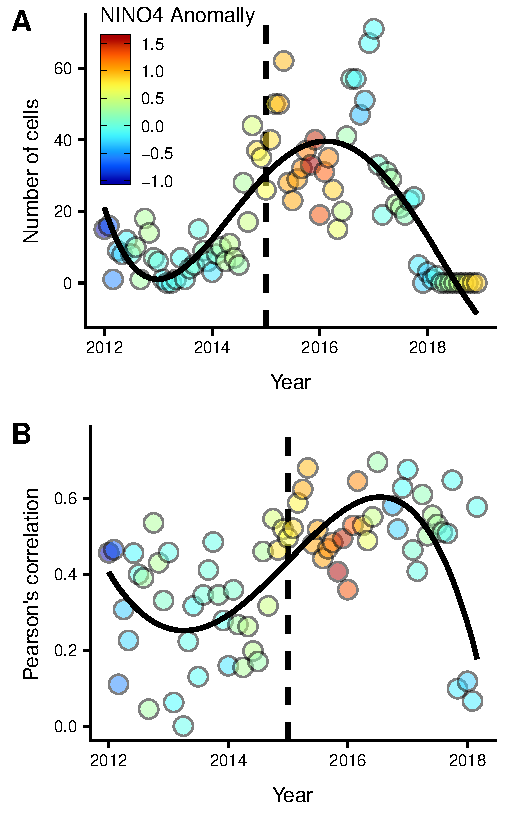
\includegraphics{img/KIR_sp_corr.pdf}
\caption{\label{fig:KIR_sp_corr}Number of cells that had displaced and non-displaced vessels (A) and spatial correlation in the presence-absence of each group per cell (B) for Kiribati's EEZ only. The solid lines represent the 4\textsuperscript{th} degree polynomial fit reported in \ref{tab:sp_corr}. Note that the late 2016 and early 2017 showed negative or neutral NINO4 anomalies, similar to those in the pre-PIPA period.}
\end{figure}

\clearpage

\bibliography{references}
\bibliographystyle{nature}

\end{document}
